The work in \cite{mercer22} accomplishes a few things that are necessary background components for this work. First, it introduces a way of interpreting a CWP as a set of LTL properties and defines this method rigorously. Second, it introduces a method for translating a BPMN diagram into verifiable Promela code. Lastly, it uses a practical example in healthcare to show that the Promela and LTL can be used to verify the expected behavior of the original BPMN, represented as a CWP.

\figref{fig:existingSolution} shows a diagram of the solution in \cite{mercer22}. More details on the CWP-to-LTL and BPMN-to-Promela translations are given in \secref{sec:backgroundCWP} and \secref{sec:backgroundBPMN} respectively.

\begin{figure*}[t]
  \begin{center}
    \begin{tabular}{c}
        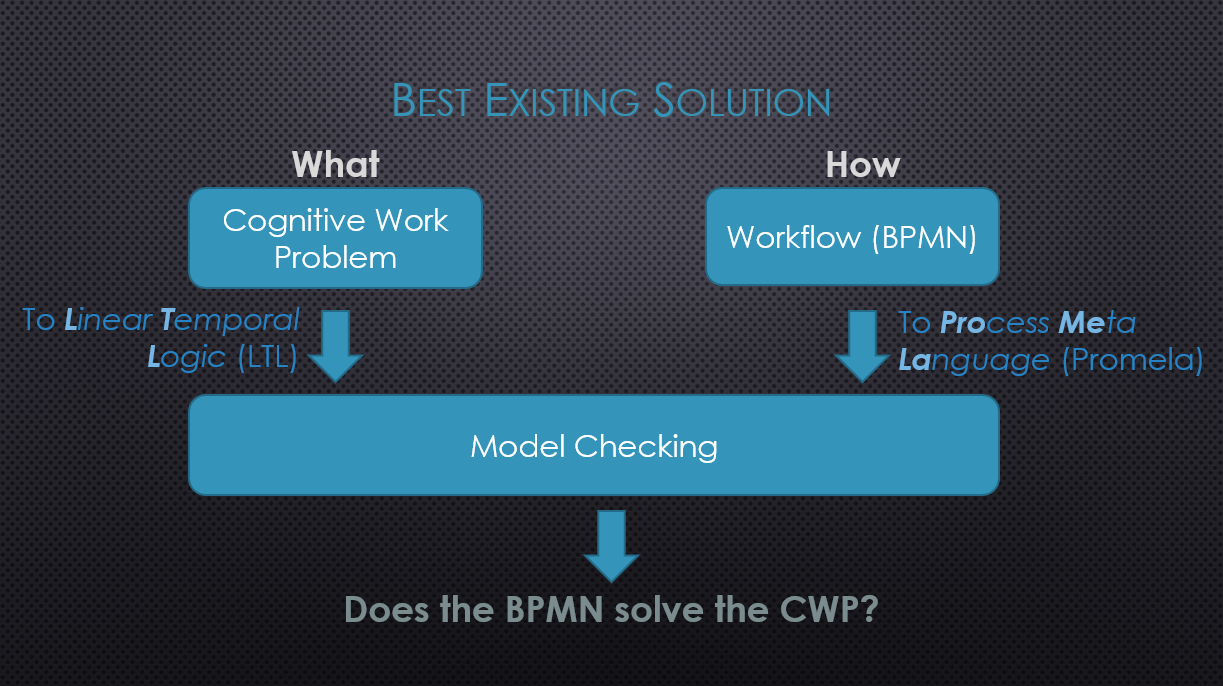
\includegraphics[width=\textwidth]{../figs/Other/ExistingSolution.png}
    \end{tabular}
  \end{center}
\caption{Diagram of the solution upon which this paper is built}
\label{fig:existingSolution}
\end{figure*}
